\documentclass[eng,printmode]{mgr}
\usepackage{polski}
\usepackage{url}
\usepackage{listings}
\usepackage[utf8]{inputenc}
\usepackage[T1]{fontenc}
\usepackage{scrextend}
\usepackage{graphicx}
\usepackage{subfigure}
\usepackage{psfrag}
\usepackage{float}
\usepackage{amsmath}
\usepackage{amsfonts}
\usepackage{enumitem}
\usepackage{supertabular}
\usepackage{array}
\usepackage{tabularx}
\usepackage{hhline}
\usepackage{graphicx}
\usepackage{showlabels}
\graphicspath{ {images/} }
\newcommand{\R}{I\!\!R}
\newtheorem{theorem}{Twierdzenie}[section]

\title{Projekt i implementacja aplikacji internetowy organizator pracy grupowej }
\engtitle{Design and implementation of web organizer for group collaboration}
\author{Maciej Bakowicz}
\supervisor{dr hab. inż. Krzysztof Walkowiak, prof. PWr, W-4}

\field{Teleinformatyka (TIN)}
\specialisation{Projektowanie sieci teleinformatycznych (TIP)}


\begin{document}
\bibliographystyle{plabbrv}

\maketitle 

\tableofcontents 

\chapter{Wstęp}  
Niniejsza praca dyplomowa opisuje liczne problemy związane z zagadnieniami dotyczącymi pracy w grupie, takimi jak problem komunikacji, wzajemnego zrozumienia czy samej organizacji, struktury a także formy kooperacji między członkami zespołu.
\\ \\
Rozdział pierwszy przedstawia zestawienie istniejących już na rynku rozwiązań, pokazuje strukturę projektu oraz opisuje wykorzystane rozwiązania i narzędzia podczas procesu implementacyjnego. Zawarte są tam także fakty oraz założenia dotyczące projektu.
\\ \\
Rozdział drugi zawiera spis wymagań funkcjonalnych wraz ze szczegółowymi opisami. Wymagania te są potrzebne do prawidłowego funkcjonowania aplikacji. Widnieje tam również podrozdział dotyczący wymagań niefunkcjonalnych zawierający m.in. wymagania dotyczące wyglądu aplikacji.
\\ \\
Rozdział trzeci przedstawia i opisuje wykonany projekt. Znajdują się tam zrzuty ekranu wraz z opisem poszczególnych części wykonanej aplikacji.
\\ \\
Końcowy, czwarty rozdział obejmuje podsumowanie całości pracy. Zawiera się w nim to co nie zostało zrealizowane oraz dalsze plany dotyczące rozwoju aplikacji w przyszłości wraz z propozycjami dodatkowych funkcjonalności . W tym rozdziale zawarte są również wnioski oraz konkluzje dotyczące procesu programistycznego oraz samego projektu aplikacji.

\section{Cel pracy}
Celem pracy jest opisanie projektu aplikacji, procesów na nią się składających oraz zaimplementowanie jej jako działającego programu rozwiązującego problemy pracy w grupie.
\\
Projekt ma zarówno wyjaśnić istniejący problem dotykający tego typu kooperacji między ludźmi a także dostarczyć gotowe rozwiązania niwelujące zaistniałe niedogodności oraz uprościć procesy powiązane z tym zagadnieniem. Głównym zadaniem jest próba poprawy mechanizmów komunikacji, systematyzacji pracy oraz podziału zadań między poszczególnych członków zespołu w sposób łatwy, wygodny a przede wszystkim efektywny, wydajny i przynoszący zyski.
\section{Problem}
Problemy wynikające z potrzeby współpracy z innymi ludźmi spotyka się zazwyczaj w sytuacjach, gdzie realizowany jest skomplikowany, obszerny projekt, wymagający znajomości wielu obszarów powiązanych ze sobą zagadnień, gdzie należy zastosować podział pracy na mniejsze fragmenty pomiędzy wielu ludzi, którzy posiadają odpowiednią wiedzę lub doświadczenie. Im większy, bardziej złożony projekt tym potrzeba podziału obowiązków jest silniejsza. Czy to wynikająca z samej struktury projektu czy innych czynników zewnętrznych takich jak ograniczenia czasowe lub jakościowe. \\
W dalszych następstwach powstają kolejne problemy, wynikające już z samej ilości zaangażowanych do projektu osób. Aby praca zespołowa przynosiła efekty musi być ona dobrze zorganizowana oraz zaplanowana.
\chapter{Analiza istniejących rozwiązań}  
\section{Badanie rynku}
Rynek aplikacji powiązanych z pracą w grupie jest bardzo obszerny. Zawierają się tam mniej lub bardziej złożone aplikacje(płatne oraz darmowe) a każda ma już spore grono odbiorców począwszy od wielkich korporacji oraz sporych rozmiarów firm po mniejsze zespoły studenckie oraz amatorskie (nie powiązane z żadną organizacją). Aplikacje te, pomimo działania w jednym obszarze biznesowym różnią się od siebie stopniem złożoności, obszerności, sposobem funkcjonowania, procesami w nich zachodzącymi czy zwyczajnie interfejsem i wyglądem.\\
Na rynku nie ma jednak oprogramowania idealnego. Każde z istniejących już rozwiązań posiada szereg wad oraz zalet. Poniższe zestawienie w sposób subiektywny opisuje powszechnie stosowane rozwiązania.
\subsection{Jira}
\begin{labeling}{Producent}
\item [Producent:] Atlassian
\item [Link:] https://pl.atlassian.com/software/jira
\end{labeling}
\subsubsection{Plusy}
\begin{itemize}
  \item[--] Wspieranie metodologii pracy(SCRUM, AGILE).
  \item[--] Integracja z wieloma systemami zewnętrznymi.
  \item[--] Stale rozwijany i usprawniany.
  \item[--] Bardzo popularny wśród większych firm, korporacji.
\end{itemize}
\subsubsection{Minusy}
\begin{itemize}
  \item[--] Nieprzejrzysty i nieintuicyjny interfejs.
  \item[--] Rozwiązanie jest całkowicie płatne .
  \item[--] Zbyt duża ilość funkcji powoduje dezorientację; Nie odpowiednie. rozwiązanie przymałych projektach.
  \item[--] Ilość funkcjonalności oraz ruchu na serwerach powoduje, że aplikacja działa wolno.
\end{itemize}

\subsection{ZenHub}
\begin{labeling}{Producent}
\item [Producent:] Zenhub
\item [Link:] https://www.zenhub.com/
\end{labeling}
\subsubsection{Plusy}
\begin{itemize}
  \item[--] Wspieranie metodologii pracy(AGILE).
  \item[--] Integracja z wieloma systemami zewnętrznymi.
  \item[--] Bezpośrednie połączenie z systemem Github.
  \item[--] Stale rozwijany i usprawniany.
\end{itemize}
\subsubsection{Minusy}
\begin{itemize}
  \item[--] Nieintuicyjny interfejs.
  \item[--] Darmowa wersja oprogramowania jest ograniczona.
  \item[--] By w pełni korzystać z serwisu należy wykupić licencję.
  \item[--] Zbyt duża ilość funkcji powoduje dezorientację; Nie odpowiednie rozwiązanie przy małych projektach.
  \item[--] Dostęp jedynie przez przeglądarkę na bezpośredniej stronie projektu w serwisie Github.
  \item[--] Przy publicznym projekcie(darmowym) na Github każdy ma wgląd do spisu zadań.
  \item[--] Ograniczenie tylko dla Github.
\end{itemize}

\subsection{Trello}
\begin{labeling}{Producent}
\item [Producent:] Trello (potem wykupione przez Atlassian)
\item [Link:] https://trello.com/
\end{labeling}
\subsubsection{Plusy}
\begin{itemize}
  \item[--] Integracja z wieloma systemami zewnętrznymi.
  \item[--] Prosty w obsłudze.
  \item[--] Intuicyjny interfejs.
\end{itemize}
\subsubsection{Minusy}
\begin{itemize}
  \item[--] Brak wsparcia dla metodologii pracy (SCRUM, AGILE itd.).
  \item[--] Darmowa wersja oprogramowania jest ograniczona.
  \item[--] By w pełni korzystać z serwisu należy wykupić licencję.
  \item[--] Projekt po zmianie właściciela nie jest już rozwijany.
  \item[--] Niektóre integracje są bardzo ograniczone i niewystarczające.
\end{itemize}

\subsection{Meister Task}
\begin{labeling}{Producent}
\item [Producent:] Meister Labs
\item [Link:] https://www.meistertask.com/
\end{labeling}
\subsubsection{Plusy}
\begin{itemize}
  \item[--] Integracja z wieloma systemami zewnętrznymi.
  \item[--] Bardzo przejrzysty i intuicyjny interfejs.
  \item[--] Świetne rozwiązania niespotykane nigdzie indziej (grafy).
\end{itemize}
\subsubsection{Minusy}
\begin{itemize}
  \item[--] Brak wsparcia dla metodologii pracy (SCRUM, AGILE itd.).
  \item[--] Darmowa wersja oprogramowania jest bardzo ograniczona.
  \item[--] Integracje dla wersji bezpłatnej są słabej jakości.
  \item[--] By w pełni korzystać z serwisu należy wykupić licencję.
  \item[--] Projekt wprowadza zmiany bardzo rzadko.
  \item[--] Niektóre integracje są bardzo ograniczone i niewystarczające.
\end{itemize}

\section{Zastosowane technologie}
\subsection{Struktura aplikacji}
Zaprojektowana aplikacja została podzielona na trzy główne części ze względu na cel oraz środowisko działania. Każda z nich została zaprojektowana w sposób autonomiczny, niezależny od pozostałych. Oznacza to, że można je traktować w sposób modularny, taki, który pozwala w bezinwazyjny dla aplikacji sposób zamienić je na inne rozwiązanie. Jedyną niezmienną rzeczą jest sposób w jaki poszczególne części się ze sobą komunikują i wymieniają dane. 
\subsubsection{Warstwa frontendowa}
Warstwa odpowiadająca za obsługę części widocznej dla użytkownika aplikacji. Ma ona za zadanie obsługę zdarzeń wykonywanych przez użytkownika takich jak gesty myszki(kliknięcia, najeżdżanie kursorem, użycie klawiatury), przełączanie między podstronami a także wyświetlanie żądanej treści. Odpowiada również za układ na stronie, wygląd poszczególnych elementów, pozycję względem innych.
\\
Warstwa ta odpowiada także za wysyłanie żądań HTTP do zewnętrznych oraz wewnętrznych serwisów w celu pozyskania oraz przetworzenia otrzymanych danych. W skład zadań dotyczących tego zagadnienia wchodzi obsługa części błędów, mogących się pojawić podczas korzystania z aplikacji.
\subsubsection{Warstwa backendowa}
Warstwa ta zajmuje się częścią po stronie serwera, nie jest ona bezpośrednio widoczna dla użytkownika. Zadaniem tej warstwy jest nasłuchiwanie i odbieranie zapytań (np. HTTP) z zewnątrz, wliczając w to poprzednią warstwę frontendową. Zajmuje się ona także połączeniem z serwisem bazodanowym, odbieraniu oraz wysyłaniu danych w ramach przetwarzania konkretnych zapytań (w zależności od zaimplementowanego systemu bazodanowego).
\\
Odbywają się tu także takie procesy jak uwierzytelnianie oraz podtrzymywanie sesji już zalogowanego użytkownika. Implementuje również obsługę błędów, głównie związanych z połączaniem bazodanowym.
\\
Warstwa ta ma za zadanie również serwować dane na zewnątrz aplikacji w formie API (Application Programming Interface - Interfejs Programowania Aplikacji)\cite{API}. Oznacza to, że w momencie przejścia pod konkretny adres aplikacji (co jest jednoznaczne z wysłaniem zapytania) jako informację zwrotną otrzymamy żądane dane w formacie JSON(JavaScript Object Notation)\cite{JSON}. Dane te można potem w dowolny sposób wykorzystać.
\\
Została tutaj zaimplementowana także forma zabezpieczenia niektórych warstw danych przed nieautoryzowanym dostępem.
\subsubsection{Warstwa systemu bazodanowego}
Warstwa systemu bazowego odpowiada za implementację oraz stworzenie fizycznej bazy danych na podstawie struktury danych. Do bazy danych łączy się warstwa backendowa posiadając odpowiednie dane autentykujące, takie jak nazwa bazy danych, adres serwera, nazwa oraz hasło użytkownika. Dane te są ustalane przez programistę.
\\
W odpowiedniku fizycznym tej warstwy są przechowywane wszelkie dane aplikacji.

\subsection{Struktura danych}
Poniżej znajdują się tabele odzwierciedlające zaimplementowaną strukturę danych. Wszelkie relacje wynikają z założeń i są tworzone dopiero po stronie warstwy backendowej. Nie istnieje logiczne powiązanie w bazie danych. Nazwy są w języku angielskim (w takim zostały zaimplementowane). Do każdej struktury automatycznie jest dołączane pole "\_id" typu String, zawierające unikalny identyfikator. Wynika to z użycia bazy MongoDB.


\begin{table}[H]
\centering
\begin{minipage}{.4\textwidth}
\paragraph{Użytkownik} \ \\ \\
\begin{tabular}{|l|l|l|}
  \hline 
  \textbf{Nazwa} & \textbf{Typ} & \textbf{Relacja}\\
  \hline
  username & String & -\\
  \hline
  email & String & -\\
  \hline
  slug & String & -\\
  \hline
  password & String & -\\
  \hline
  tasks & Array & Zadanie\\
  \hline
  createdAt & Date & -\\
  \hline
\end{tabular} 
\caption{Struktura danych użytkownika}
\end{minipage}\hfill
\begin{minipage}{.4\textwidth}
\paragraph{Projekt} \ \\ \\
\begin{tabular}{|l|l|l|}
  \hline 
  \textbf{Nazwa} & \textbf{Typ} & \textbf{Relacja}\\
  \hline
  name & String & -\\
  \hline
  description & String & -\\
  \hline
  slug & String & -\\
  \hline
  members & Array & Użytkownik\\
  \hline
  boards & Array & Tablica\\
  \hline
  createdAt & Date & -\\
  \hline
\end{tabular} 
\caption{Struktura danych projektu}
\end{minipage}\hfill
\end{table}

\begin{table}[H]
\centering
\begin{minipage}{.4\textwidth}
\paragraph{Tablica} \ \\ \\
\begin{tabular}{|l|l|l|}
  \hline 
  \textbf{Nazwa} & \textbf{Typ} & \textbf{Relacja}\\
  \hline
  name & String & -\\
  \hline
  icon & String & -\\
  \hline
  slug & String & -\\
  \hline
  tasks & Array & Zadanie\\
  \hline
  project & Array & Projekt\\
  \hline
  createdAt & Date & -\\
  \hline
\end{tabular} 
\caption{Struktura danych tablicy}
\end{minipage}\hfill
\begin{minipage}{.4\textwidth}
\paragraph{Zadanie} \ \\ \\
\begin{tabular}{|l|l|l|}
  \hline 
  \textbf{Nazwa} & \textbf{Typ} & \textbf{Relacja}\\
  \hline
   name & String & -\\
  \hline
   description & String & -\\
  \hline
   isDone & Boolean & -\\
  \hline
   prior & Number & -\\
  \hline
   order & Number & -\\
  \hline
   slug & String & -\\
  \hline
   chat & String & Czat\\
  \hline
   author & String & Użytkownik\\
  \hline
   assigned & Array & Użytkownik\\
  \hline
   board & String & Tablica\\
  \hline
   createdAt & Date & -\\
  \hline
\end{tabular} 
\caption{Struktura danych zadania}
\end{minipage}\hfill
\end{table}

\begin{table}[H]
\centering
\begin{minipage}{.4\textwidth}
\paragraph{Czat} \ \\ \\
\begin{tabular}{|l|l|l|}
  \hline 
  \textbf{Nazwa} & \textbf{Typ} & \textbf{Relacja}\\
  \hline
   name & String & -\\
  \hline
   description & String & -\\
  \hline
   type & String & -\\
  \hline
   project & String & Projekt\\
  \hline
   members & Array & Użytkownik\\
  \hline
   createdAt & Date & -\\
  \hline
\end{tabular} 
\caption{Struktura danych czatu}
\end{minipage}\hfill
\begin{minipage}{.4\textwidth}
\paragraph{Wiadomość czatu} \ \\ \\
\begin{tabular}{|l|l|l|}
  \hline 
  \textbf{Nazwa} & \textbf{Typ} & \textbf{Relacja}\\
  \hline
   message & String & -\\
  \hline
   chat & String & Czat\\
  \hline
   author & String & Użytkownik\\
  \hline
   createdAt & Date & -\\
  \hline
\end{tabular} 
\caption{Struktura danych wiadomości czatu}
\end{minipage}\hfill
\end{table}
\newpage

\subsection{Języki programistyczne}
Warstwa frontendowa została napisana w języku JavaScript\cite{JS}, z wykorzystaniem standardu EcmaScript 6\cite{ES6} oraz składni TypeScript\cite{TS}. Dodatkowo został użyty język znaczników HTML5 ( HyperText Markup Language)\cite{HTML5}, który służy do reprezentacji treści, jaką przeglądarka internetowa jest w stanie interpretować oraz kaskadowych arkuszy styli CSS3 (Cascading Style Sheets)\cite{CSS3}, dzięki którym możliwym było stworzenie przejrzystego interfejsu. Użycie znaczników HTML 5 sprawiło na dodatek, że aplikacja jest przygotowana do pozycjonowania SEO(Search Engine Optimization)\cite{HTML_SEO} a wdrożenie najnowszych funkcjonalności CSS3, takich jak animacje oraz obsługa niektórych zdarzeń myszki zwiększyło szybkość ładowania się aplikacji, gdyż nie potrzebna jest implementacja po stronie języka JavaScript, który obciąża łącze internetowe oraz procesor\cite{JS_CPU}. Kolejnym atutem jest fakt, iż nawet przy wyłączonej obsłudze JavaScript przeglądarki, aplikacja nadal będzie w pewien sposób używalna (chociażby po to, żeby móc poinformować użytkownika o konieczności włączenia obsługi JavaScript).
\\
\\
Warstwa backendowa również została zaimplementowana w języku JavaScript (z zastosowaniem EcmaScript 6 oraz TypeScript). Posiadanie tego samego języka programowania w obu tych warstwach niesie szereg zalet, z których najważniejszą jest czytelność kodu, poprzez podobne implementacje funkcjonalności na obu tych warstwach, co sprawia, że kod czytany przez osoby trzecie jest łatwiej i szybciej zrozumieć. Jest to niezwykle ważne w dalszych procesach rozwojowych, w chwili gdy zajdzie potrzeba powiększenia zespołu programistycznego.
\\
Dodatkowym atutem jest możliwość użycia podobnych (jeśli nie tych samych) narzędzi programistycznych oraz konfiguracji środowiska.
\\
\\
System bazodanowy wykorzystuje implementację MongoDB\cite{MongoDB}, która to posiada strukturę bazy typu NoSQL\cite{NO_SQL}. System ten jest bardzo prosty do skomunikowania z wykorzystującą język JavaScript warstwę backendową. Baza danych MongoDB wykorzystuje notację JSON. Nie implementuje powiązań typowych dla np. MySQL, gdzie występują klucze obce oraz relacje. Każda struktura danych jest z założenia nie powiązana z żadną inną (w sensie implementacyjnym, po stronie samego systemu MongoDB). Sposób relacji zatem określa się dopiero po stronie programowej(tu: warstwa backendowa) i jest on dowolny, optymalnie dobrany do potrzeb i sytuacji.

\subsection{Wykorzystane rozwiązania}

Poniżej zostały opisane najważniejsze technologie / rozwiązania użyte w projekcie wraz z przykładem zakresu pracy, który dotyczą. W częśc niektórych zastosowanych rozwiązań wchodzą pomniejsze biblioteki, które wykorzystując nadrzędne rozwiązanie implementują dodatkowe funkcjonalności. Te pomniejsze biblioteki, nie zostały w jawny sposób opisane, gdyż często ich wkład ogranicza się jedynie do formy interpretacji kodu lub formy w jaki jest on napisany. Ich spis znajduje się w postaci tabel w odpowiednich paragrafach.

\subsubsection{Preprocessor Sass}
Język Sass i preprocessor z nim związany\cite{Sass} wprowadza nowy sposób w jaki kod CSS jest pisany. Wraz z inną architekturą kodu wprowadza szereg dodatkowych funkcjonalności, takie jak instrukcje warunkowe, pętle, funkcje. Głównym plusem stosowania preprocessora Sass jest zmniejszenie objętości wymaganego do napisania kodu. Dodatkowo zbliżenie do natury języka typowo programistycznego sprawia, że pisanie jest dużo bardziej intuicyjne.

\subsubsection{React.js}
React.js\cite{React} został wykorzystany w aplikacji jako podstawa warstwy frontendowej. Wykorzystuje koncepcję tworzenia komponentów JavaScript, dzięki czemu kod napisany jest bardzo modularny i reużywalny. Do samego frameworka zostały użyte dodatkowe biblioteki.

\begin{table}[H]
\begin{tabularx}{\textwidth}{|X|X|}
  \hline
    \textbf{Nazwa} & \textbf{Wersja} \\
  \hline
   	react-dom & 16.0.0 \\
  \hline
  	react-fa & 5.0.0 \\
   \hline
   	react-moment & 0.6.5 \\
   \hline
  	react-redux & 5.0.6 \\
   \hline
  	react-router & 4.2.0 \\
   \hline
  	react-router-dom & 4.2.2 \\
   \hline
  	react-sortable-hoc & 0.6.8 \\
   \hline
   reselect & 3.0.1 \\
   \hline
\end{tabularx}
\caption{Biblioteki wykorzystywane przez React}
\end{table}

\subsubsection{Redux}
Redux\cite{Redux} jest rozszerzeniem do React.js, pozwalającym na lepszą organizację kodu poprzez automatyzację części funkcjonalności. Wraz z samym rozszerzeniem używane są dodatkowe biblioteki wspomagające pracę Redux.

\begin{table}[H]
\begin{tabularx}{\textwidth}{|X|X|}
   \hline
    \textbf{Nazwa} & \textbf{Wersja} \\
   \hline
    redux-actions & 2.2.1 \\
   \hline
   	redux-axios & 0.0.2 \\
   \hline
  	redux-axios-middleware & 4.0.0 \\
   \hline
   	redux-devtools-extension & 2.13.2 \\
   \hline
  	redux-saga & 0.15.6 \\
   \hline
\end{tabularx}
\caption{Biblioteki wykorzystywane przez Redux}
\end{table}


\subsubsection{Axios}
Axios\cite{Axios} to biblioteka JavaScript, która została wykorzystana do wysyłania zapytań HTTP na serwer(warstwa backendowa) w celu pobrania danych w notacji JSON.

\subsubsection{Socket.io}
Socket.io\cite{SocketIO} to biblioteka implementująca koncepcję Web Socket\cite{Keyword_Websocket}. Została użyta po stronie warstwy frontendowej oraz backendowej w celu zapewnienia komunikacji w czasie rzeczywistym podczas działania zaimplementowanego komunikatora. Rozwiązanie te pozwala na dosyć istotną redukcję ilości wysyłanych i odebranych zapytań w aplikacji poprzez obsługę tylko zdarzeń, które rzeczywiście miały miejsce. Eliminuje to problem cyklicznego "odpytywania" warstwy backendowej w celu sprawdzenia czy baza danych została zmieniona.

\subsubsection{Sortable.js}
Bilbioteka Sortable.js\cite{SortableJS} to obszerne narzędzie do zarządzania elementami typu "przeciągnij oraz upuść"(tzw. Drag and Drop). Została zaimplementowana w celu podniesienia poziomu User Experience\cite{Keyword_UserExperience}.

\subsubsection{Moment.js}
Biblioteka ta\cite{MomentJS} służy do formatowania daty, odliczania czasu. Została zaimplementowana w miejscach gdzie nastąpiła referencja do daty stworzenia elementu.

\subsubsection{Node.js}
Struktura oparta o Node.js\cite{NodeJS} jest wykorzystywana jako główny filar warstwy backendowej. Framework ten jest odpowiedzialny za całą obsługę serwera oraz wcześniej opisanych (patrz: warstwa backendowa) funkcjonalności. Dodatkowo oprogramowanie oferuje system zarządzania zależnościami (NPM, patrz: wykorzystane narzędzia).

\subsubsection{Express}
Express\cite{Express} jest rozszerzeniem wzbogacającym oprogramowanie Node.js o dodatkowe funkcjonalności automatyzujące oraz usprawniające pisanie kodu.

\begin{table}[H]
\begin{tabularx}{\textwidth}{|X|X|}
   \hline
    \textbf{Nazwa} & \textbf{Wersja} \\
   \hline
     body-parser & 1.17.2 \\
   \hline
     jsonwebtoken & 8.1.0 \\
   \hline
  	 jwt-decode & 2.2.0 \\
   \hline
   	 mongoose & 4.11.8 \\
   \hline
\end{tabularx}
\caption{Biblioteki wykorzystywane przez Express}
\end{table}

\subsection{Wykorzystane narzędzia}

\subsubsection{Node Package Manager (NPM)}
Node Package Manager (NPM)\cite{NPM} jest dostarczanym wraz z oprogramowaniem Node.js narzędziem do zarządzania zależnościami projektowymi. Przez te pojęcie rozumie się wszelkie zewnętrzne paczki dodatkowych bibliotek, rozszerzeń programistycznych. NPM pozwala na proste ich dodawanie, usuwanie oraz aktualizację w zależności od potrzeb (np. dotyczących wersji).

\subsubsection{Yarn}
Yarn\cite{Yarn} jest dodatkową paczką wspierającą oraz rozszerzającą NPM o funkcjonalności głównie dotyczących  zainstalowanych już paczek. Jest wykorzystywany w projekcie do kontrolowania wersji zależności (automatyzacja wyszukiwania nieaktualnych oraz ich aktualizacja za pomocą jednej komendy). Dzięki Yarn można także sprawdzić, które paczki są nieużywane w projekcie (co determinuje możliwość ich usunięcia).

\subsubsection{Sass Lint}
Zależność ta\cite{SassLint} wspomaga proces zachowania czystego, bardziej czytelniejszego kodu napisanego w preprocessorze  Sass poprzez stosowanie (wcześniej zdefiniowanych) zasad dotyczących np. ilości spacji, odstępów tabulatora, sposobu zapisania reguł. Proces ten nosi nazwę lintowania.

\subsubsection{TS Lint}
TypeScript Linter\cite{TSLint} ma analogiczne zadanie co wyżej wymieniony Sass Lint, jednak dotyczy kodu zapisanego w języku TypeScript.

\subsubsection{Webpack}
Webpack\cite{Webpack} jest narzędziem sprawującym kontrolę nad automatyzacją wielu zadań dotyczących kodu oraz środowiska programistycznego. Do głównych zadań należy przede wszystkim transpilacja\cite{Keyword_Transpile}, czyli tłumaczenia języka napisanego przez programistę na inną jego wersję, co tu przekłada się na przepisywanie kodu w standardzie ES6(który nie jest zrozumiały przez przeglądarki) na standard ES5, który jest w pełni kompatybilny z interpretatorem przeglądarek. Kod napisany w preprocesorze Sass również jest niezrozumiały dla przeglądarek, toteż webpack zajmuje się transpilacją na język kaskadowych arkuszy stylów CSS.
\\
W narzędziu tym możemy zdefiniować dodatkowe reguły dotyczące pliku wyjściowego, m.in.: łączenie wszystkiego w jeden plik (bundle), zmiana nazw zmiennych w celu zaoszczędzenia miejsca, zmiana nazw klas CSS wg. ustalonego schematu oraz wiele innych. 
\\
Webpack wykorzystuje dużo gotowych rozwiązań podczas swojej pracy.

\begin{table}[H]
\begin{tabularx}{\textwidth}{|X|X|}
   \hline
    \textbf{Nazwa} & \textbf{Wersja} \\
   \hline
     awesome-typescript-loader & 3.2.3 \\
   \hline
     source-map-loader & 0.2.2 \\
   \hline
     style-loader & 0.19.0 \\
   \hline
  	 to-string-loader & 1.1.5 \\
   \hline
   	 ts-loader & 2.3.4 \\
   \hline
   	 sass-loader & 6.0.6 \\
   \hline
   	 raw-loader & 0.5.1 \\
   \hline
   	 node-sass & 4.5.3 \\
   \hline
   	 css-loader & 0.28.7 \\
   \hline
     extract-text-webpack-plugin & 3.0.1 \\
   \hline
     file-loader & 1.1.5 \\
   \hline
     html-webpack-plugin & 2.30.1 \\
   \hline
     url-loader & 0.6.2 \\
   \hline
     webpack-node-externals & 1.6.0 \\
   \hline
\end{tabularx}
\caption{Biblioteki wykorzystywane przez Webpack}
\end{table}
   
\subsubsection{Nodemon}
Nodemon\cite{Nodemon} jest wsparciem do zarządzania serwerem podczas procesu programowania. Rozwiązuje on problem potrzeby ciągłego odświeżania domyślnego serwera dostarczanego przez oprogramowanie Node.js w chwili zmiany pliku, który jest aktualnie przetwarzany. Nodemon w prosty sposób wprowadza nasłuch na zmiany tego pliku, automatycznie restartując serwer gdy takowe się pojawią.

\subsubsection{GIT}
System kontroli wersji GIT\cite{GIT} w folderze plików aplikacji tworzy repozytorium, w którym możemy tworzyć gałęzie (branch) zawierające tylko zmiany na plikach wykonanych w jej obrębie. Przekłada się to na wysokiej jakości kontrolę nad zawartością kodu oraz zwiększeniu bezpieczeństwa wynikającego z błędu programistycznego. 

\subsubsection{Travis CI}
Travis CI \cite{TravisCI} jest to narzędzie typu Continuous Integration \cite{Keyword_CI} pozwalające na kontrolowanie wysyłanego kodu na serwis Github. Narzędzie to nasłuchuje na zdarzenia typu "push" (webhook \cite{Keyword_Webhook}) i w momencie zarejestrowania uruchamia szereg komend(zdefiniowanych przez programistę) wykonujących się na kodzie. Te etapy to między innymi proces budowania aplikacji (build), uruchamianie narzędzie ts/sass lint (lint) oraz przesyłanie kodu na serwis Heroku(deploy) w celu ponownego uruchomienia aplikacji na serwerze zdalnym z zastosowaniem nowych funkcjonalności. \\
Zapewnia to, że wykonany do pewnego etapu projekt jest w pełni funkcjonalny, wolny od błędów programistycznych czy kodowych. Travis CI wspiera wysyłanie powiadomień (np. e-mail) w chwili gdy którykolwiek z etapów nie zostanie wykonany poprawnie co minimalizuje czas potrzebny na naprawę aplikacji.

\subsubsection{Heroku}
Heroku\cite{Heroku} jest to darmowa platforma do uruchamiania aplikacji na serwerze(dostarczanym przez Heroku). Dzięki temu projekt jest możliwy do podglądu online. Dodatkowo Heroku tworzy repozytorium wraz z kodem aplikacji, co zabezpiecza kod przez utraceniem (głównym repozytorium pozostaje Github). Platforma ta dostarcza również wgląd w statystyki aplikacji oraz logi zawierające takie informacje jak status aplikacji, historię nawiązywanych połączeń oraz zdarzeń. Usprawnia to proces ewentualnego wyszukiwania błędów programistycznych.

\subsubsection{Baza danych seriwsu mLab}
W projekcie została wykorzystana darmowa implementacja bazy danych MongoDB udostępniana przez serwis mLab (https://mlab.com/). Nie było zatem konieczne instalowania serwisu bazy danych na komputerze lokalnym(podczas procesu programowania). Jednocześnie dane używane podczas implementacji są takie same jak w chwili udostępnienia podglądu online na platformę Heroku.

\subsubsection{Github}
Github (http://www.github.com) jest internetową platformą pozwalającą na magazynowanie kodu aplikacji za pomocą oprogramowania GIT. Stosowanie tego rozwiązania zabezpiecza kod aplikacji przed utraceniem wskutek czynników trzecich. Zapewnia także jej mobilność (możliwość uruchomienia oraz programowania na dowolnym urządzeniu bez potrzeby angażowania fizycznych nośników danych).
\\
\\

\begin{table}[H]
\begin{tabularx}{\textwidth}{|X|X|}
   \hline
    \textbf{Nazwa} & \textbf{Wersja} \\
   \hline
      axios & 0.16.2 \\
   \hline
     express & 4.15.4 \\
   \hline
  	  lodash & 4.17.4 \\
   \hline
   	  moment & 2.19.1 \\
   \hline
   	 normalize.css & 7.0.0 \\
   \hline
   	 normalize.css & 7.0.0 \\
   \hline
   	 react & 16.0.0 \\
   \hline
   	 redux & 3.7.2 \\
   \hline
   	 sass-lint & 1.12.0 \\
   \hline
   	 socket.io & 2.0.4 \\
   \hline
   	  socket.io-client  & 2.0.4 \\
   \hline
      sortablejs & 1.6.1 \\
   \hline
     tslint & 5.7.0 \\
   \hline
      tslint-react & 3.2.0 \\
   \hline
      typescript & 2.5.3 \\
   \hline
     webpack & 3.7.1 \\
   \hline
\end{tabularx}
\caption{Spis wersji wykorzystanych rozwiązań/narzędzi oraz innych wykorzystywanych globalnie paczek (nie uwzględnionych w powyższym zestawieniu).}
\end{table}

\section{Fakty i założenia związane z projektem }
\begin{itemize}
  \item Do prawidłowego funkcjonowania aplikacji potrzebne jest połączenie z Internetem.
  \item Niektóre sieci nie zezwalają na połączenia z serwisem Heroku oraz mLab.
  \item Aby korzystać z niektórych narzędzi należy posiadać konta w niektórych wymienionych serwisach.
  \item Żadne z zastosowanych rozwiązań / narzędzi nie jest płatne.
  \item Kod aplikacji znajduje się w publicznym repozytorium serwisu Github.
  \item Aplikacja jest napisana w języku angielskim.
\end{itemize}
\chapter{Wymagania dotyczące projektu}

\section{Wymagania funkcjonalne}

\subsection{Implementacja API}
\begin{labeling}{Nr wymagania}
\item [Nr wymagania:] 1
\item [Priorytet:] Wymagane
\end{labeling}

\subsubsection{Przesłanka}
W celu udostępnienia danych za pomocą struktury systemu API należy stworzyć ścieżki (routes), na adresy których wysyłane są zapytania HTTP w celu otrzymania wiadomości zwrotnej zawierającej odpowiedni fragment danych, wyspecyfikowany w ścieżce url.

\subsubsection{Interesariusze}
Wszyscy użytkownicy oraz dla części danych użytkownicy zalogowani, posiadający odpowiednie uprawnienia, zdeterminowane odpowiednimi przynależnościami do struktur.

\subsubsection{Opis}
Po odebraniu zapytania na konkretnym adresie warstwa backendowa uruchamia wcześniej zaimplementowane funkcje, które łączą się z warstwą bazodanową i w zależności od typu żądania wykonuje odpowiednie akcje:
\begin{itemize}
  \item[--] \textbf{GET}: Po odebraniu zapytania funkcja zwraca wszystkie rekordy żądanego typu a następnie są one wysyłane jako wiadomość zwrotna.
  \item[--] \textbf{GET SINGLE}: Po odebraniu tego typu żądania funkcja zwraca tylko zdefiniowane dane konkretnego obiektu (na podstawie parametru w adresie url) a następnie są one wysłane jako wiadomość zwrotna.
  \item[--] \textbf{POST}: Funkcja sprawdza czy wszystkie pola zdefiniowane w bazie danych jako wymagane zawierają się w obiekcie przysłanym pod odebrany adres oraz czy są one poprawne (pod względem typu, unikalności, wielkości). Gdy nie wystąpiły problemy odebrane dane są wysyłane do warstwy systemu bazodanowego, gdzie następuje ich zapis jako nowego rekordu.
  \item[--] \textbf{PUT}: Proces analogiczny jak dla żądania typu POST, jednak wymagany jest parametr identyfikujący konkretny, już istniejący obiekt (przekazany w ścieżce) w bazie danych. Dodatkowo, gdy element przysłanego obiektu jest już zdefiniowany (istnieje w obiekcie w bazie) zostaje on podmieniony na ten nadesłany w zapytaniu.
  \item[--] \textbf{DELETE}: Zapytanie to wymaga przekazania parametru identyfikującego w adresie ścieżki (url). Gdy obiekt istnieje w bazie danych zostaje on z niej usunięty.
\end{itemize}
\ \\
Ścieżki (routes) są zdefiniowane na podstawie schematu:
\begin{itemize}
  \item[--] \textbf{POST, GET}: /api/\textit{nazwa-struktury-danych}, np: /api/user
  \item[--] \textbf{GET SINGLE, PUT, DELETE}: /api/\textit{nazwa-struktury-anych}/\textit{parametr-identyfikujący}, np: /api/user/john-smith.
\end{itemize}
Dodatkowo nie wszystkie typy zapytań oraz ścieżki są dostępne dla każdego użytkownika aplikacji. Użytkownik niezalogowany ma dostęp tylko do:
\begin{itemize}
  \item [--] Istniejących użytkowników(adres e-mail, nazwa użytkownika).
  \item[--] Istniejących projektów(nazwa projektu).
\end{itemize}
\ \\
Każdy zalogowany użytkownik otrzymuje dostęp do:
\begin{itemize}
  \item[--] Swoich danych (bez pola password, które nie jest przesyłane w żadnej formie jako odpowiedź ze strony serwera).
  \item[--] Danych do projektu, na bazie którego wykonał akcję logowania (dane projektu + dane powiązane takie jak współużytkownicy, tablice, zadania).
\end{itemize}
\ \\
Autoryzacja jest zaimplementowana z wykorzystaniem tokenu JWT\cite{Keyword_JWTToken}.

\subsection{Implementacja ścieżki dla warstwy frontendowej}
\begin{labeling}{Nr wymagania}
\item [Nr wymagania:] 2
\item [Priorytet:] Wymagane
\end{labeling}

\subsubsection{Przesłanka}
Aby możliwa była obsługa aplikacji przy pomocy interfejsu graficznego, warstwa backendowa musi posiadać informacje o konieczności wyświetlenia odpowiedniego pliku na konkretnej ścieżce.


\subsubsection{Interesariusze}
Wszyscy użytkownicy.

\subsubsection{Opis}
Po odebraniu zapytania na adres główny domeny (adres nie posiadający żadnych parametrów w ścieżce url) serwer (warstwa backendowa) wyświetla dokument o nazwie index.html jako statyczny plik. Rozszerzenie pliku sprawi, że nie potrzeba wykonywać dodatkowych akcji, ponieważ przeglądarka poprawnie zinterpretuje zawartą w pliku treść. \\
Dodatkowo, aby zezwolić na pobieranie innych plików statycznych (obrazy, czcionki) przez przeglądarkę na podobnej zasadzie jest zaimplementowana ścieżka pod adresem '/static'.

\subsection{Rejestracja nowego konta}
\begin{labeling}{Nr wymagania}
\item [Nr wymagania:] 3
\item [Priorytet:] Wymagane
\end{labeling}

\subsubsection{Przesłanka}
Aby korzystać z funkcjonalności jakie oferuje aplikacja należy posiadać założone konto. Korzystanie z aplikacji wymaga uwierzytelnienia. Wiele funkcjonalności użytkowych musi być powiązane z inicjatorem zdarzenia / wykonanej akcji, takie jak przypisanie użytkownika jako autora do pewnych stworzonych struktur.

\subsubsection{Interesariusze}
Potencjalni użytkownicy aplikacji, użytkownicy nieposiadający zarejestrowanego konta w serwisie.

\subsubsection{Opis}
W celu umożliwienia korzystania z aplikacji nowym użytkownikom należy stworzyć formularz rejestracyjny na nowej podstronie z wymaganymi polami:
\begin{itemize}
	\item[--] Nazwa nowego lub istniejącego projektu.
	\item[--] Nazwa konta użytkownika.
	\item[--] Hasło użytkownika.
	\item[--] Potwierdzenie hasła użytkownika.
\end{itemize}
\ \\
Wszystkie pola wymagają poprawnej walidacji pod kątem poprawności danych według następujących zasad:
\begin{itemize}
	\item[--] Żadne pole nie może być puste.
	\item[--] Pole z nazwą projektu(w sytuacji gdy nie istnieje) oraz nazwą użytkownika musi mieć co najmniej 6 znaków oraz być unikalne(inne od już stworzonych).
	\item[--] Pole z nazwą projektu(w sytuacji gdy istnieje) musi być powiązane z adresem e-mail użytkownika(poprzez wcześniejsze manualne powiązanie).
	\item[--] Pole z hasłem użytkownika musi mieć co najmniej 7 znaków oraz zawierać co najmniej jedną cyfrę.
	\item[--] Pole z hasłem użytkownika oraz potwierdzeniem muszą być identyczne.
\end{itemize}
\ \\
Podczas próby wysłania formularza z błędnie wypełnionymi polami powinna pojawić się zawierająca treść błędów informacja.
\\
Gdy pola zostaną zweryfikowane (sprawdzone pod kątem poprawności) poprawnie, po wysłaniu formularza zostanie wprowadzony nowy rekord do bazy danych zawierający dane nowego użytkownika a sam użytkownik zostanie automatycznie przekierowany na stronę logowania. Dodatkowo, gdy wpisany projekt nie został odnaleziony w bazie danych tworzony jest nowy. Nowo stworzony użytkownik zostaje jednocześnie członkiem tego projektu.

\subsection{Logowanie do aplikacji}
\begin{labeling}{Nr wymagania}
\item [Nr wymagania:] 4
\item [Priorytet:] Wymagane
\end{labeling}

\subsubsection{Przesłanka}
Zalogowanie się do serwisu zapewnia dostęp do wszystkich funkcjonalności aplikacji.

\subsubsection{Interesariusze}
Wszyscy użytkownicy posiadający aktywne konto w serwisie.

\subsubsection{Opis}
Proces logowania polega na wypełnieniu formularza na stronie głównej następującymi danymi:
\begin{itemize}
	\item[--] Nazwa projektu.
	\item[--] Nazwa użytkownika.
	\item[--] Hasło użytkownika.
\end{itemize}
\ \\
Po wysłaniu formularza aplikacja sprawdza zgodność wprowadzonych danych z danymi zaimplementowanymi w bazie danych. Weryfikuje się czy:
\begin{itemize}
	\item[--] Użytkownik o podanej nazwie istnieje.
	\item[--] Hasło użytkownika jest poprawne.
	\item[--] Nazwa projektu zawiera się w bazie danych.
	\item[--] Użytkownik należy do projektu.
\end{itemize}
\ \\
W przypadku niepowodzenia wyświetlany jest komunikat o niepoprawnych danych. W przypadku sukcesu strona główna się odświeża a strona logowania jest podmieniana przez stronę główną aplikacji dostępnej dla zalogowanego użytkownika. Dodatkowo token JWT zawierający zakodowane dane takie jak nazwa użytkownika oraz projektu jest zapisywany w bazie danych przeglądarki typu Local Storage\cite{Keyword_LocaLStorage}.

\subsection{Wyświetlanie statystyk strony}
\begin{labeling}{Nr wymagania}
\item [Nr wymagania:] 5
\item [Priorytet:] Wymagane
\end{labeling}

\subsubsection{Przesłanka}
Wgląd do ilości zawartej w projekcie treści takiej jak ilość zadań, stworzonych tablic czy użytkowników  usprawnia proces pracy z użyciem aplikacji. Posiadanie wiedzy dotyczącej obecnej sytuacji projektu pomaga szybciej oszacować etap, w którym projekt się znajduje, co jednoznacznie przekłada się na możliwość dostosowania pracy zalogowanego użytkownika do współpracowników.

\subsubsection{Interesariusze}
Wszyscy użytkownicy posiadający aktywne konto w serwisie, jednocześnie zalogowani do serwisu. Użytkownicy powiązani tym samym projektem.

\subsubsection{Opis}
Strona statystyk ma formę kilku tabel zawierających ostatnie pięć rekordów dotyczących odpowiedniej treści w niej prezentowanej, takiej jak lista ostatnio dodanych użytkowników oraz lista ostatnio stworzonych zadań. Pod każdą z tabel znajduje się przycisk sugerujący rozszerzenie ilości treści prezentowanej w danej tabeli.
\\
Dla tabeli zawierającej zadania przycisk ten przekierowuje użytkownika na podstronę z tablicami oraz zadaniami.
\\
Dla tabeli zawierającej listę użytkowników po naciśnięciu owego przycisku lista ta zostaje rozwinięta o kolejne pięć pozycji. Po pierwszym rozwinięciu pojawia się kolejny przycisk sugerujący ukrycie właśnie rozwiniętych elementów. W sytuacji gdy tabela zawiera wszystkie rekordy (lista wszystkich użytkowników) przycisk umożliwiający zwiększanie widocznych pozycji znika.
\\ \\
Na stronę statystyk składają się również trzy boksy z ilością odpowiednich danych. Osobny boks dla: liczby zadań, liczby tablic, liczby użytkowników.

\subsection{Strona z tablicami oraz zadaniami}
\begin{labeling}{Nr wymagania}
\item [Nr wymagania:] 6
\item [Priorytet:] Wymagane
\end{labeling}

\subsubsection{Przesłanka}
Priorytetowym celem aplikacji jest umożliwienie tworzenia oraz zarządzania tablicami i zadaniami dotyczącymi projektu. Odpowiednia ich wizualizacja jest konieczna do zapewnienia intuicyjnej oraz prostej pracy w aplikacji.

\subsubsection{Interesariusze}
Wszyscy użytkownicy posiadający aktywne konto w serwisie, jednocześnie zalogowani do serwisu. Użytkownicy powiązani tym samym projektem.

\subsubsection{Opis}
Projekt domyślnie nie posiada żadnych tablic oraz zadań, toteż strona odwiedzana po raz pierwszy prezentuje jedynie przycisk umożliwiający dodanie nowej tablicy wraz z widoczną informacją odnośnie potrzeby wykonania tej akcji. \\
Strona ze stworzonymi już tablicami oraz zadaniami ma formę kilku kolumn, które reprezentują kolejne stworzone tablice. Ilość kolumn jest zdeterminowana ilością tablic. Każda kolumna składa się z ikony, nazwy oraz panelu opcji tablicy. W panelu rozwijanym znajduje się opcja usunięcia tablicy. \\
Poniżej w formie listy znajdują się stworzone zadania, wraz z tytułem oraz skróconym opisem do 120 widocznych znaków. Dodatkowo w formie koloru opisany jest priorytet zadania. Jeśli tablica nie posiada przypisanych zadań wówczas widoczny jest komunikat o konieczności stworzenia lub przypisania już istniejącego (z innej tablicy). Na dole każdej listy znajduje się przycisk umożliwiający dodanie nowego zadania.

\subsection{Dodawanie nowej tablicy}
\begin{labeling}{Nr wymagania}
\item [Nr wymagania:] 7
\item [Priorytet:] Wymagane
\end{labeling}

\subsubsection{Przesłanka}
Wymagane jest dostosowanie środowiska aplikacji do potrzeb projektu w celu zapewnienia optymalnej pracy.

\subsubsection{Interesariusze}
Wszyscy użytkownicy posiadający aktywne konto w serwisie, jednocześnie zalogowani do serwisu. Użytkownicy powiązani tym samym projektem.

\subsubsection{Opis}
Po naciśnięciu odpowiedniego przycisku otworzy się formularz zawierający pola z:
\begin{itemize}
  \item[--] Nazwą nowej tablicy.
  \item[--] Listą rozwijaną z ikonami.
\end{itemize}
\ \\
Wymagane jest aby pole z nazwą nowej tablicy było wypełnione. Gdy nie zostanie wybrana żadna ikona, jest wybierana ikona domyślna. Gdy wystąpił błąd pojawia się informacja zawierająca jego treść. W przypadku sukcesu zostaje wysłane odpowiednie zapytanie do API, zawierające dane tablicy oraz dołączone z bazy Local Storage informacje dotyczące nazwy projektu. W warstwie backendowej następuje proces wprowadzenia nowej tablicy do bazy danych.
\newpage

\subsection{Edycja istniejącej tablicy}
\begin{labeling}{Nr wymagania}
\item [Nr wymagania:] 8
\item [Priorytet:] Wymagane
\end{labeling}

\subsubsection{Przesłanka}
W czasie projektu mogą wystąpić zmiany w organizacji i strukturze tablic. 

\subsubsection{Interesariusze}
Wszyscy użytkownicy posiadający aktywne konto w serwisie, jednocześnie zalogowani do serwisu. Użytkownicy powiązani tym samym projektem.

\subsubsection{Opis}
Po naciśnięciu nazwy tablicy w widoku tablic pojawi się kursor umożliwiający dynamiczną zmianę nazwy tablicy (edycja za pomocą pola tekstowego). Pole z nazwą tablicy nie może być puste. Tablica zostanie zaktualizowana w momencie kliknięcia poza obszar nazwy lub klawisza Enter.
\\
Po kliknięciu na ikonę przy nazwie tablicy pojawi się lista rozwijana z dostępnymi ikonami do wyboru. Po kliknięciu na którąś z nich ikona zostanie od razu zaktualizowana a lista zamknięta. Listę można zamknąć też bez wybierania ikony poprzez kliknięcie poza jej obszar.

\subsection{Usuwanie istniejącej tablicy}
\begin{labeling}{Nr wymagania}
\item [Nr wymagania:] 9
\item [Priorytet:] Wymagane
\end{labeling}

\subsubsection{Przesłanka}
W czasie projektu mogą wystąpić zmiany w organizacji i strukturze tablic.

\subsubsection{Interesariusze}
Wszyscy użytkownicy posiadający aktywne konto w serwisie, jednocześnie zalogowani do serwisu. Użytkownicy powiązani tym samym projektem.

\subsubsection{Opis}
Z listy rozwijanej obok nazwy tablicy, po wyborze opcji dotyczącej usuwania, pojawi się komunikat wymagający potwierdzenia tej akcji z informacją o ewentualnych skutkach. Jeśli do tablicy przypisane są jakieś zadania wówczas  komunikat ten zawiera opcję (w formie pola wyboru) dotyczącą losu obecnych zadań. Pole to zawiera dwie opcje, z którą jedną z nich jest permanentne usunięcie przypisanych do tablicy zadań a drugą możliwość przypisania do innej tablicy (jeśli istnieje). Po potwierdzeniu usunięcia tablicy wykonywane są wybrane akcje.

\subsection{Dodawanie nowego zadania}
\begin{labeling}{Nr wymagania}
\item [Nr wymagania:] 10
\item [Priorytet:] Wymagane
\end{labeling}

\subsubsection{Przesłanka}
Lista zadań jest głównym celem istnienia aplikacji

\subsubsection{Interesariusze}
Wszyscy użytkownicy posiadający aktywne konto w serwisie, jednocześnie zalogowani do serwisu. Użytkownicy powiązani tym samym projektem.

\subsubsection{Opis}
Po naciśnięciu przycisku pod listą zadań w widoku tablicy pojawia się formularz z następującymi polami:
\begin{itemize}
  \item[--] Nazwą zadania.
  \item[--] Opisem zadania.
  \item[--] Listą wyboru priorytetu.
  \item[--] Opcją z możliwością otworzenia detali tego zadania po jego dodaniu.
\end{itemize}
Pole z nazwą oraz opisem nie może być puste, dodatkowo nazwa zadania musi być unikalna. Priorytet jest domyślnie ustawiony na najwyższy a opcja otworzenia dodatkowych informacji zaznaczona.\\
Po zatwierdzeniu formularza zadania zostanie ono dodane i w zależności od wybranej opcji pojawia się okno ze szczegółami tego zadania (widok zarządzania zadaniem). Autorem zostaje inicjator akcji. Zadanie jest przypisywane do tablicy, z której przycisk dotyczący dodania został naciśnięty. Zadanie otrzymuje najwyższą liczbę w kolejności (jako ostatnie).

\subsection{Sortowanie oraz organizacja zadań}
\begin{labeling}{Nr wymagania}
\item [Nr wymagania:] 11
\item [Priorytet:] Wymagane
\end{labeling}

\subsubsection{Przesłanka}
Odpowiednia wizualizacja kolejności oraz dystrybucji zadań pomiędzy różnymi tablicami poprawia przejrzystość projektu oraz usprawnia pracę.

\subsubsection{Interesariusze}
Wszyscy użytkownicy posiadający aktywne konto w serwisie, jednocześnie zalogowani do serwisu. Użytkownicy powiązani tym samym projektem.

\subsubsection{Opis}
Zmiana kolejności zadań oraz przypisania do innej tablicy odbywa się za pomocą mechanizmu Drag \& Drop (przeciągnij i upuść). Kolejność jest determinowana odpowiednim atrybutem w bazie danych, który po wykonaniu każdej tego typu akcji jest aktualizowany. W momencie przypisania (przenoszenie pomiędzy tablicami) zmienia się również atrybut zadania wskazujący przynależność do tablicy. Gdy zostanie przeniesione ostatnie zadanie z listy pojawia się komunikat (na liście) informujący o braku zadań i konieczności stworzenia lub ponownego przypisania.

\subsection{Widok zarządzania zadaniem}
\begin{labeling}{Nr wymagania}
\item [Nr wymagania:] 12
\item [Priorytet:] Wymagane
\end{labeling}
\subsubsection{Przesłanka}
Edycja stworzonym wcześniej zadaniem poprawia przejrzystość projektu. Wytyczne do zadania mogą się zmieniać w czasie.

\subsubsection{Interesariusze}
Wszyscy użytkownicy posiadający aktywne konto w serwisie, jednocześnie zalogowani do serwisu. Użytkownicy powiązani tym samym projektem.

\subsubsection{Opis}
Po krótkim naciśnięciu na zadanie widoczne na liście w pojedynczej tablicy otwiera się okno ze szczegółami zadania wraz z możliwością ich edytowania:
\begin{itemize}
  \item[--] Nazwa oraz opis zadania jest edytowana w formie dynamicznej, za pomocą zmiany bezpośrednio w polu ich wyświetlenia (na podstawie pola tekstowego, opisane w wymaganiu nr 8).
  \item[--] Przyciski dotyczące usuwania zadania oraz zaznaczania jako wykonane są odblokowane tylko dla osoby przypisanej do tego zadania.
  \item[--] Zmiana przypisania użytkowników do zadania jest dozwolona tylko przez autora.
\end{itemize}
Zawarte są również informacje o autorze, dacie stworzenia zadania oraz tablicy, do której jest ono przypisane. \\
Dodatkowo znajduje się tam również okno czatu. W zależności od zadania może być to tylko przycisk, informujący o możliwości stworzenia systemu wiadomości lub już stworzony czat z wiadomościami. Każdy tego typu czat jest również dostępny z poziomu widoku czatu (wymaganie nr  13).\\
Okno zarządzania zadaniem jest zamykane po naciśnięciu odpowiedniego przycisku.
\newpage

\subsection{Widok czatu wiadomości tekstowych}
\begin{labeling}{Nr wymagania}
\item [Nr wymagania:] 13
\item [Priorytet:] Wymagane
\end{labeling}

\subsubsection{Przesłanka}
Wymagana jest komunikacja w obrębie projektu między użytkownikami w celu efektywnej pracy i ustalania szczegółów dotyczących projektu.

\subsubsection{Interesariusze}
Wszyscy użytkownicy posiadający aktywne konto w serwisie, jednocześnie zalogowani do serwisu. Użytkownicy powiązani tym samym projektem. Czasami użytkownicy mający uprawnienia do odpowiedniego czatu.

\subsubsection{Opis}
W każdym nowo stworzonym projekcie domyślnie jest tworzony czat o nazwie "random" (z ang. losowy, dowolny). W założeniu czat ten ma się tyczyć rozmów na dowolny temat. \\
Typy czatów możemy podzielić na publiczne (mają do niego dostęp wszyscy powiązani z projektem użytkownicy), prywatny (dostęp tylko dla zaproszonych użytkowników), task (dostęp dla osób powiązanych z konkretnym zadaniem).
\\
Widok czatu składa się z listy chronologicznie posortowanych wiadomości(najnowsza na dole), pola tekstowego z możliwością dodania wiadomości oraz spisu wszystkich dostępnych dla użytkownika czatów z podziałem na te dotyczące zadań oraz inne. Po kliknięciu na któryś widocznych na liście okno z wiadomościami zmienia się. Dodatkowo na dole listy czatów (niedotyczących zadań) znajduje się przycisk do stworzenia nowego pokoju (chatroom, z ang. kanał dyskusyjny).

\subsection{Stworzenie nowego pokoju czatu}
\begin{labeling}{Nr wymagania}
\item [Nr wymagania:] 14
\item [Priorytet:] Wymagane
\end{labeling}

\subsubsection{Przesłanka}
Tworzenie nowych pokoi czatu jest przydatne i konieczne w celu wymiany zdań na tematy niezwiązane z zadaniami. Podział i organizacja jest ważnym aspektem dotyczącym przejrzystości i efektywności pracy.

\subsubsection{Interesariusze}
Wszyscy użytkownicy posiadający aktywne konto w serwisie, jednocześnie zalogowani do serwisu. Użytkownicy powiązani tym samym projektem.

\subsubsection{Opis}
Po naciśnięciu odpowiedniego przycisku wyświetla się formularz zawierający pola z:
\begin{itemize}
  \item[--] Nazwą pokoju.
  \item[--] Opcjonalnego opisu.
  \item[--] Typu(publiczny, prywatny).
  \item[--] Listy z użytkownikami, którzy otrzymają dostęp do uczestnictwa w dyskusji (tylko opcja prywatna).
\end{itemize}
Żadne z pól nie może być puste (poza opisem). Domyślnie typ czatu jest ustawiony na publiczny. Nie ma limitu uczestników przypisanych do czatu prywatnego.
\\
Po zatwierdzeniu formularza czat zostaje utworzony a autor (inicjator) przekierowany na stronę z nowo powstałym pokojem.

\subsection{Stworzenie nowej wiadomości tekstowej}
\begin{labeling}{Nr wymagania}
\item [Nr wymagania:] 15
\item [Priorytet:] Wymagane
\end{labeling}

\subsubsection{Przesłanka}
Tworzenie wiadomości tekstowych jest podstawą funkcjonowaniem czatu wiadomości.

\subsubsection{Interesariusze}
Wszyscy użytkownicy posiadający aktywne konto w serwisie, jednocześnie zalogowani do serwisu. Użytkownicy powiązani tym samym projektem. Użytkownicy mający dostęp do pokoju (chatroom).

\subsubsection{Opis}
Po zatwierdzeniu wiadomości wpisanej w odpowiednim polu(patrz wymaganie nr 13) pojawia się ona na samym dole listy wiadomości.
\\
Wiadomość składa się z nazwy autora, daty utworzenia, awataru(tu: graficznej formy reprezentacji) użytkownika.

\subsection{Widok profilu użytkownika}
\begin{labeling}{Nr wymagania}
\item [Nr wymagania:] 16
\item [Priorytet:] Wymagane
\end{labeling}

\subsubsection{Przesłanka}
Personalizacja profilu oraz podgląd aktywności swojej oraz innych pozytywnie wpływa na organizację i przypisywanie zadań. 

\subsubsection{Interesariusze}
Wszyscy użytkownicy posiadający aktywne konto w serwisie, jednocześnie zalogowani do serwisu.

\subsubsection{Opis}
Strona profilu użytkownika składa się z listy zawierającej podstawowe informacje o użytkowniku, takie jak nazwa, adres e-mail, data dołączenia do projektu, liczbę stworzonych zadań oraz liczbę zadań przypisanych. \\
Kolejną częścią profilu jest podzielona na trzy części lista zadań. Każda cześć zawiera odpowiednio przefiltrowane zadania, których użytkownik jest autorem bądź został do niego przypisany. Odpowiednio są to: wszystkie zadania, zadania ukończone, zadania nieukończone. \\
Właściciel profilu, podglądając swój własny może w prosty sposób edytować informacje takie jak nazwa użytkownika, adres e-mail czy hasło (edycja przebiega na takiej samej zasadzie co edycja tytułu tablicy - wymaganie nr 8).

\subsection{Wysyłanie zaproszeń do projektu}
\begin{labeling}{Nr wymagania}
\item [Nr wymagania:] 17
\item [Priorytet:] Wymagane
\end{labeling}

\subsubsection{Przesłanka}
W skład projektu często wchodzi więcej niż jeden użytkownik.

\subsubsection{Interesariusze}
Wszyscy użytkownicy posiadający aktywne konto w serwisie, jednocześnie zalogowani do serwisu.

\subsubsection{Opis}
Każdy zalogowany do projektu użytkownik ma możliwość wysłania zaproszenia niezarejestrowanemu lub zarejestrowanemu ale nie przypisanemu do projektu(tego do którego zaproszenie jest wysyłane) użytkownikowi. Z głównego menu wybierana jest opcja dotycząca wysyłaniu nowego zaproszenia, po naciśnięciu której pojawia się formularz z dwoma polami:
\begin{itemize}
  \item[--] Polem tekstowym przeznaczonym na ręczne wpisanie adresu e-mail
  \item[--] Polem wyboru z listą zarejestrowanych już użytkowników(ale nie przypisanych do projektu aktywnego)
\end{itemize}
Po wybraniu adresu e-mail na podstawie jednego z pól (wypełnienie jednego z nich automatycznie blokuje możliwość wypełnienia drugiego) zależnie od tego, czy w bazie danych znajduje się podany adres, czy nie, podejmowana jest jedna z akcji:
\begin{itemize}
  \item[--] Jeśli użytkownik o podanym adresie e-mail istnieje otrzymuje on powiadomienie (możliwa implementacja powiązana z wymaganiem nr 18) lub wiadomość wysłaną na ten adres.
  \item[--] Jeśli adres e-mail nie znajduje się w bazie danych, generowane jest losowe hasło (losowy ciąg znaków), które zostaje  wysłane na adres e-mail wraz z podstawowymi informacjami o projekcie.
\end{itemize}

\subsection{System powiadomień}
\begin{labeling}{Nr wymagania}
\item [Nr wymagania:] 18
\item [Priorytet:] Niewymagane
\end{labeling}

\subsubsection{Przesłanka}
Dokumentowanie akcji związanych z projektem oraz użytkownikiem w znacznym stopniu usprawnia procesy zarządzania zadaniami, tablicami i ogólnie projektem. Umożliwia to na przykład szybsze reagowanie na podejmowane przez innych użytkowników akcje, takie jak zmiany w zadaniach, wiadomości w czacie.

\subsubsection{Interesariusze}
Wszyscy użytkownicy posiadający aktywne konto w serwisie, jednocześnie zalogowani do serwisu.

\subsubsection{Opis}
Po naciśnięciu odpowiedniego przycisku pojawia się panel boczny z wylistowanymi zdarzeniami dotyczącymi użytkownika. Jedno zdarzenie zawiera takie informacje jak data, zakres, typ. W zależności od typu zdarzenia możliwe są dodatkowe akcje takie jak np. odnośnik do zadania/czatu, którego zdarzenie dotyczy.

\section{Wymagania niefunkcjonalne}
\subsection{Wymaganie estetyczne}
\begin{itemize}
  \item Styl aplikacji musi być utrzymany w konwencji Material Design\cite{Material}
  \item Aplikacja musi spełniać standardy narzucone przez serwis MDN\cite{MDN_HTML}\cite{MDN_CSS} dotyczących użycia znaczników HTML5 oraz CSS3.
  \item Interfejs aplikacji musi spełniać podstawowe założenia ideii User Experience oraz User Interface\cite{Keyword_UserInterface}.
  \item Aplikacja zakłada przejrzystość struktury oraz estetykę interfejsu.
\end{itemize} 

\subsection{Wymaganie dotyczące ergonomii i wygody}
\begin{itemize}
  \item Korzystanie z aplikacji nie powinno wymagać znajomości użytych języków programistycznych czy ogólnie pojętego programowania.
  \item Wszelkie interakcje ze strukturą interfejsu aplikacji powinny przebiegać dynamicznie, bez zbędnych przekierowań na podstrony  czy oczekiwania na rezultat wykonanych akcji.
\end{itemize}
\subsection{Wymagania dotyczące skalowalności i rozszerzalności}
\begin{itemize}
  \item Dodawanie nowych funkcjonalności do aplikacji nie powinno być procesem skomplikowanym, ingerującym za bardzo w napisany kod.
  \item Struktura MongoDB jest stworzona z myślą o przetrzymywaniu dużej ilości danych, toteż graniczne wartości liczbowe dotyczące ilości konkretnych danych nie są możliwe do ustalenia. Należy jednak pamiętać, że w celu obsługi dużej ilości użytkowników przetwarzających dane wymagany jest również serwer o odpowiednio dobranej mocy obliczeniowej.
  \item Użyte środowisko programistyczne nie jest przygotowane do obsługi aplikacji w wersji finalnej. Wymaganym jest zatem, aby finalna wersja aplikacji była zaimplementowana w komercyjnym, odpowiednio dobranym środowisku.
\end{itemize}
\subsection{Wymagania dotyczące bezpieczeństwa korzystania z systemu}
\begin{itemize}
  \item System bazodanowy musi być odpowiednio zabezpieczony przed ingerencją osób nieautoryzowanych. Wymaga się zatem aby hasło zabezpieczające posiadało znaki różnego typu (litery, cyfry, znaki specjalne)
  \item Wymagane jest, aby baza danych aplikacji w wersji finalnej była zaimplementowana w odpowiednio przygotowanym środowisku, oferującym rozwiązania wysokiej jakości oraz zabezpieczenia w postaci kopi zapasowych. Nie zaleca się stosowania rozwiązań darmowych, w których bezpieczeństwo przed utratą danych jest niezapewnione.
  \item W bazie danych nie mogą być przetrzymywane jawne hasła. Należy zapewnić zabezpieczenie w postaci użycia funkcji korzystającej z MD5\cite{MD5} lub pochodnej.
\end{itemize}
\chapter{Projekt aplikacji}
\section{Opis aplikacji}
Poniżej znajduje się opis najważniejszych funkcjonalności zaimplementowanej aplikacji.
\subsection{Strona główna przed zalogowaniem}

\subsubsection{Widok strony logowania}
\begin{figure}[H]
  \begin{center}
  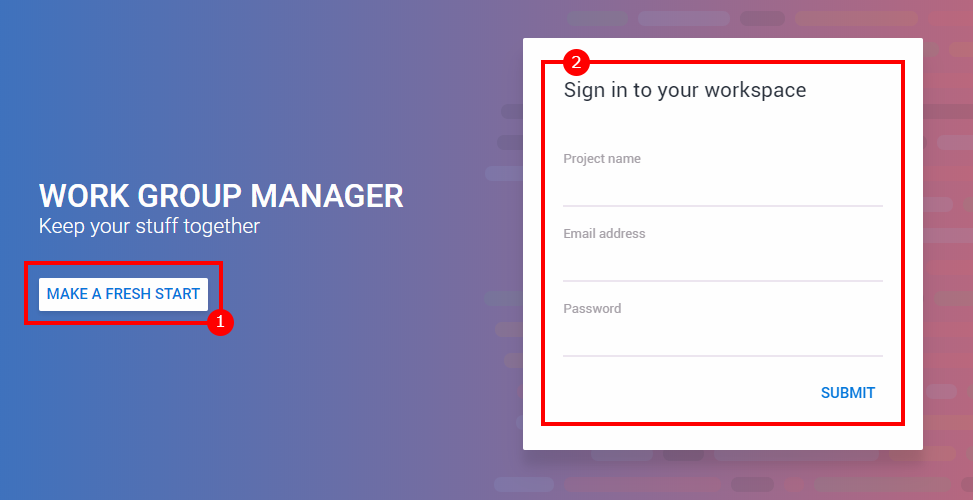
\includegraphics[scale=0.62]{login}
  \end{center}
  \caption{Widok strony głównej przed zalogowaniem}
\end{figure}

\begin{enumerate}
  \item Link do strony rejestracji.
  \item Formularz umożliwiający zalogowanie się do serwisu.
\end{enumerate}
\newpage

\subsubsection{Widok strony rejestracji}
\begin{figure}[H]
  \begin{center}
  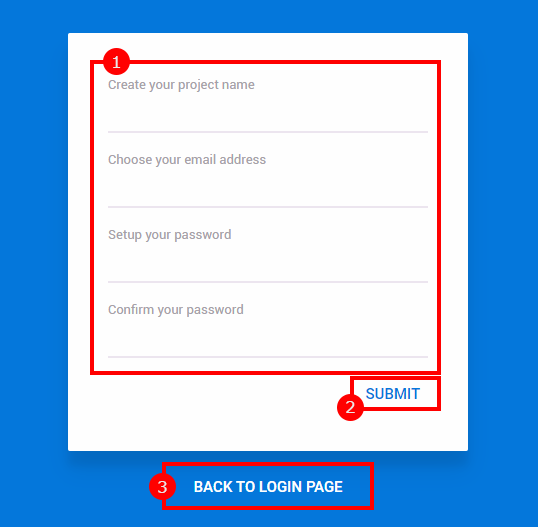
\includegraphics[scale=0.8]{register}
  \end{center}
  \caption{Widok strony rejestracji nowego konta}
\end{figure}

\begin{enumerate}
  \item Pola wymagane w celu zarejestrowania nowego konta w serwisie. 
  \item Przycisk wysyłający formularz.
  \item Link umożliwiający powrót do strony logowania.
\end{enumerate}
\newpage

\subsection{Strona główna po zalogowaniu}
\subsubsection{Menu}
\begin{figure}[H]
  \begin{center}
  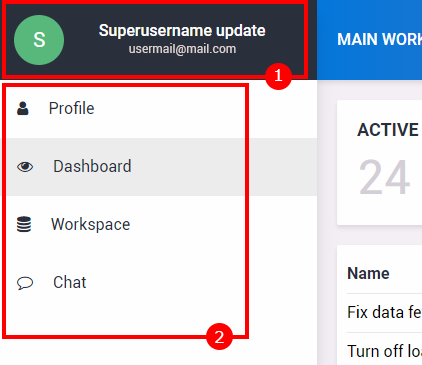
\includegraphics[scale=0.8]{menu}
  \end{center}
  \caption{Widok menu aplikacji}
\end{figure}

\begin{enumerate}
  \item Podgląd zalogowanego użytkownika. Widoczne informacje: wygenerowany awatar, nazwa użytkownika, adres e-mail.
  \item Spis dostępnych zakładek wraz z ikonami.
\end{enumerate}
\newpage

\subsubsection{System powiadomień}
\begin{figure}[H]
  \begin{center}
  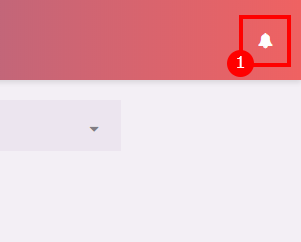
\includegraphics[scale=0.8]{notification}
  \end{center}
  \caption{Widok ikony włączającej panel powiadomień}
\end{figure}

\begin{enumerate}
  \item Ikona włączająca system powiadomień.
\end{enumerate}
\newpage

\subsubsection{Statystyki strony}
\begin{figure}[H]
  \begin{center}
  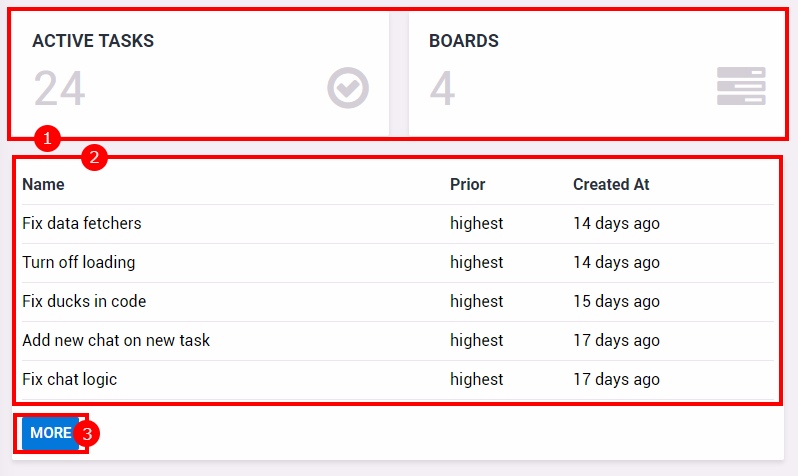
\includegraphics[scale=0.75]{stats}
  \end{center}
  \caption{Widok statystyk}
\end{figure}
\begin{enumerate}
  \item Liczbowe podsumowanie treści na stronie wraz z podpisem oraz ikoną.
  \item Spis pięciu ostatnio dodanych zadań.
  \item Przycisk przekierowujący do widoku tablic i zadań.
\end{enumerate}
\newpage

\subsection{Widok tablic oraz zadań}
\subsubsection{Widok dodawania tablicy}
\begin{figure}[H]
  \begin{center}
  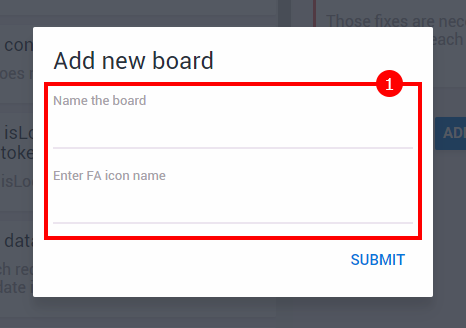
\includegraphics[scale=0.8]{add_board}
  \end{center}
  \caption{Widok formularza dodawania nowej tablicy}
\end{figure}
\begin{enumerate}
  \item Pola wymagane opisujące tablicę.
\end{enumerate}
\newpage

\subsubsection{Widok tablicy z zadaniami}
\begin{figure}[H]
  \begin{center}
  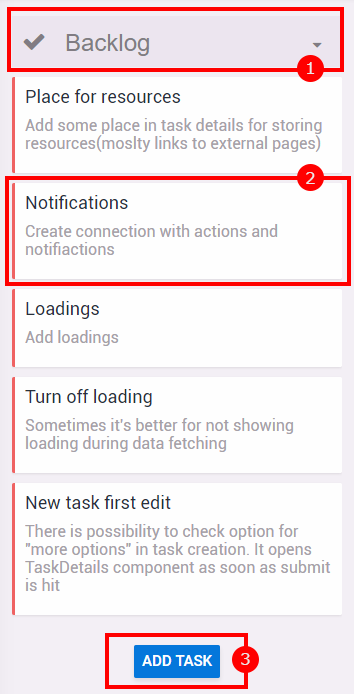
\includegraphics[scale=0.8]{task_list_board}
  \end{center}
  \caption{Widok tablicy wraz z listą zadań}
\end{figure}
\begin{enumerate}
  \item Informacje odnośnie tablicy. Od lewej: ikona, nazwa tablicy, menu z opcjami.
  \item Widok pojedynczego zadania na liście. Widoczne informacje: kolor oznaczający priorytet, nazwa zadania, opis.
  \item Przycisk umożliwiający dodanie zadania.
\end{enumerate}
\newpage

\subsubsection{Widok dodawania zadania}
\begin{figure}[H]
  \begin{center}
  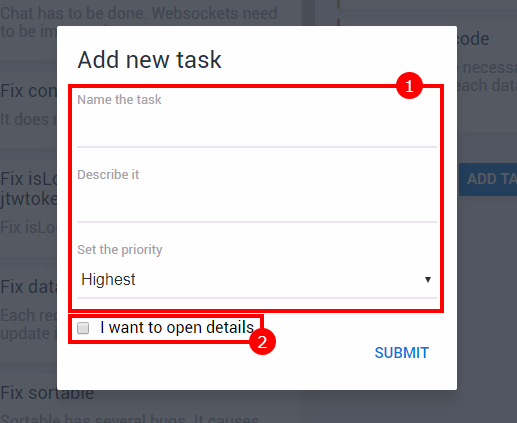
\includegraphics[scale=0.8]{add_task}
  \end{center}
  \caption{Widok formularza dodawania nowego zadania}
\end{figure}
\begin{enumerate}
  \item Pola wymagane opisujące zadanie.
  \item Pole wyboru dotyczące otwarcia szczegółów po  stworzeniu zadania.
\end{enumerate}
\newpage

\subsubsection{Widok szczegółów zadania}
\begin{figure}[H]
  \begin{center}
  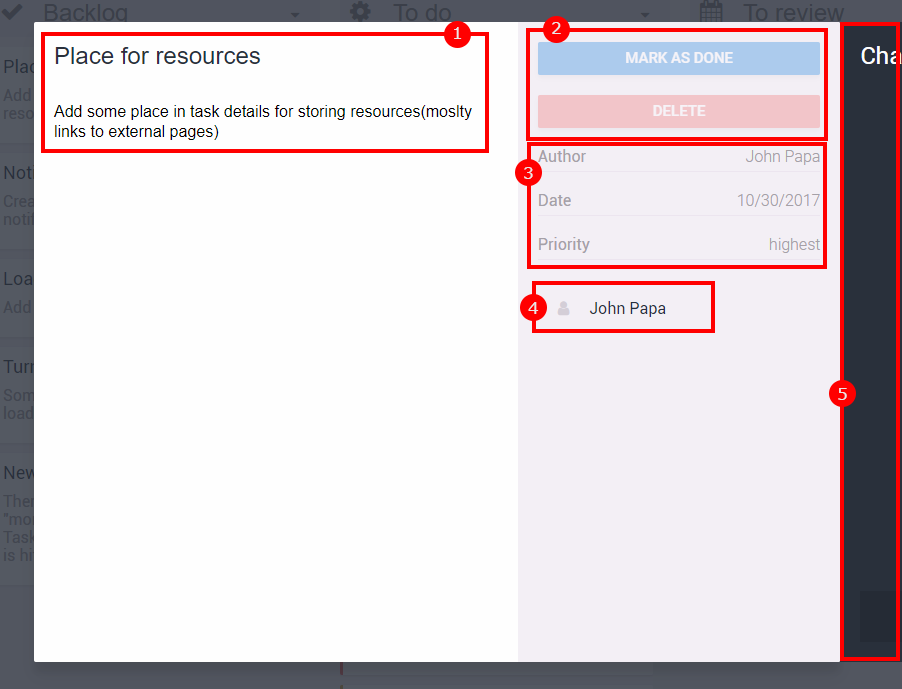
\includegraphics[scale=0.66]{task_details}
  \end{center}
  \caption{Widok szczegółów zadania}
\end{figure}
\begin{enumerate}
  \item Podstawowe informacje opisujące zadanie: Tytuł oraz opis.
  \item Przyciski do zaznaczania zadania jako wykonany oraz usuwanie w formie zablokowanej.
  \item Spis dodatkowych informacji: autor, data utworzenia, priorytet.
  \item Spis osób przypisanych do zadania.
  \item Kawałek czatu dotyczącego tego zadania.
\end{enumerate}
\newpage
\subsection{Widok czatu wiadomości tekstowych}
\subsubsection{Widok przykładowego czatu z listą wiadomości}
\begin{figure}[H]
  \begin{center}
  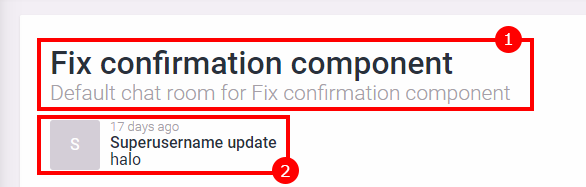
\includegraphics[scale=0.75]{chat}
  \end{center}
  \caption{Widok czatu}
\end{figure}
\begin{enumerate}
  \item Podstawowe informacje opisujące pokój czatu: Nazwa oraz opis.
  \item Widok wiadomości wysłanej na czacie zawierająca podstawowe informajce takie jak: czas, nazwę użytkownika, treść, awatar.
\end{enumerate}
\newpage

\subsubsection{Menu boczne czatu wiadomości}
\begin{figure}[H]
  \begin{center}
  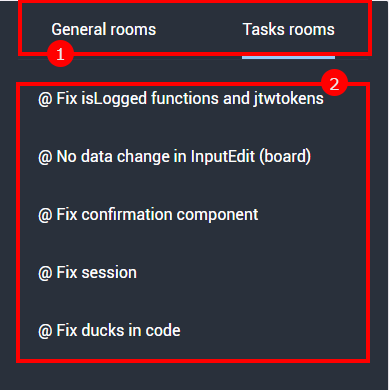
\includegraphics[scale=0.8]{task_chat_lists}
  \end{center}
  \caption{Widok menu czatu}
\end{figure}

\begin{enumerate}
  \item Podział na czaty dotyczące zadań oraz inne.
  \item Lista czatów powiązanych z zadaniami.
\end{enumerate}
\newpage

\subsection{Widok profilu użytkownika}
\subsubsection{Informacje użytkownika}
\begin{figure}[H]
  \begin{center}
  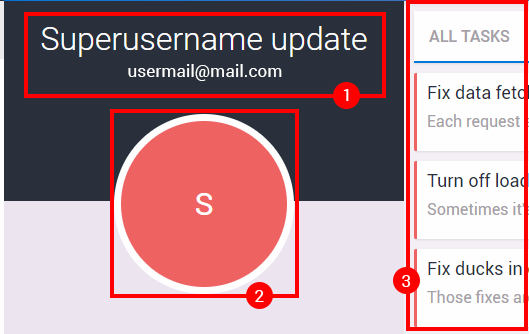
\includegraphics[scale=0.8]{profile}
  \end{center}
  \caption{Widok profilu użytkownika}
\end{figure}

\begin{enumerate}
  \item Główne informacje użytkownika takie jak nazwa oraz adres e-mail.
  \item Wygenerowany awatar.
  \item Lista zadań z zakładkami filtrującymi na podstawie statusu (wszystkie, ukończone, nieukończone).
 \end{enumerate}
\newpage

\chapter{Podsumowanie}
Implementacja projektu nie została w pełni ukończona jednak udało się spełnić większość wymagań funkcjonalnych i niefunkcjonalnych (niektóre tylko częściowo), głównie tych o priorytecie wymaganym. Wymagań o priorytecie niższym nie udało się zaimplementować wcale, jednak są one solidną podstawą pod dalszą część rozwoju aplikacji w przyszłości.
\\
Powodem był zarówno niewystarczający czas poświęcony na proces implementacyjny jak i wiele problemów napotkanych w czasie realizacji (programistycznych oraz innego typu).
\\
\\
Dobór wymienionych technologii programistycznych i narzędzi wspierających ten proces okazał się dobrym pomysłem. Błędy i niedociągnięcia wynikały tylko z przyczyn braku wystarczającej ilości czasu na nauczenie się ich a nie z faktu użycia któregoś z nich. Stosowanie tych technologii nie sprawiało problemu w zrozumieniu ich działania czy użycia.
\section{Implementacja a wymagania}
Poniżej znajduje się wypunktowana lista zawierająca to czego nie udało się zaimplementować a było wymienione w wymaganiach:
\begin{itemize}
  \item Brak zabezpieczeń przed nieautoryzowanym dostępem do danych dostępnych z poziomu API.
  \item Brak rejestracji nowego konta dla wcześniej stworzonego projektu (rejestracja tylko dla nowego). 
  \item Brak możliwości edycji ikony tablicy.
  \item Brak możliwości usuwania tablicy.
  \item Brak implementacji Drag \& Drop dla tablic w celu zmiany ich kolejności.
  \item System Drag \& Drop (przeciągnij i upuść) dla listy zadań czasami powoduje błędy w działaniu całej aplikacji (brak obsługi niektórych związanych z tą technologią błędów).
  \item Brak możliwości przypisywania innych użytkowników do zadania poza autorem.
  \item Brak obsługi niektórych błędów i zdarzeń dotyczących czatu (niechronologiczne wyświetlanie wiadomości w kilku miejscach).
  \item Brak możliwości tworzenia nowego czatu.
  \item Brak systemu zaproszeń (powiązane z drugim punktem tej listy).
  \item Brak systemu powiadomień.
\end{itemize}
Zostały jednak spełnione wszystkie wymagania dotyczące wyglądu aplikacji oraz ergonomii i wygody korzystania z niej. Aplikacja posiada przejrzysty i intuicyjny interfejs oraz jest w pełni dynamiczna pod względem zarządzania danymi czy szybkości działania. \\
Zaimplementowane wymagania funkcjonalne spełniają część zakładanej roli pomimo błędów w działaniu niektórych z nich.

\section{Problemy zaistniałe podczas implementacji}
Poniżej znajdują się najważniejsze problemy napotkane podczas realizacji projektu dyplomowego. Mają one charakter ogólny, nie zawierają konkretnych części (np. funkcji w kodzie, dni, wydarzeń):
\begin{itemize}
  \item Brak wystarczającej ilości czasu spowodowany innymi obowiązkami w czasie realizacji projektu, takie jak praca czy obowiązki szkolne.
  \item Występowanie błędów dotyczących użycia gotowych rozwiązań, brak pomysłów i wiedzy na ich rozwiązanie co spowodowane było nieznajomością wszystkich wybranych struktur, technologi, narzędzi (co jednocześnie jest powiązane z brakiem wystarczającej ilości czasu na nauczenie się ich).
\end{itemize}
\section{Plany i możliwości rozwojowe projektu}
Dalszy rozwój aplikacji w przyszłości wymagać będzie na pewno dokończenia rozpoczętych już funkcjonalności oraz niwelacji istniejących błędów. Tylko wtedy będzie można rozpocząć proces usprawniania aplikacji o dodatkowe założenia i wymagania. Głównymi pomysłami o jakie warto rozszerzyć aplikację są na pewno:
\begin{itemize}
  \item Implementacja logowania za pomocą zewnętrznych serwisów takich jak Facebook, Google, Twitter.
  \item System migracji zadań / tablic z podobnych serwisów na rynku.
  \item Wprowadzenie integracji z systemami zewnętrznymi(Github, Docker, Jenkins).
  \item Usprawnienia czatu wiadomości pod kątem wyglądu oraz implementacja możliwości przesyłania mediów takich jak obrazy, wideo, linki, dokumenty.
  \item Dodatkową integrację z systemami kontroli wersji (GIT) w celu połączenia projektu bezpośrednio z aplikacją umożliwiając tym samym przeglądanie zmian wprowadzanych przez współpracowników wraz z systemem komentarzy.
  \item Stworzenie aplikacji na telefon umożliwiającą podgląd zmian oraz nadzorowanie projektu bez potrzeby bycia stacjonarnym.
\end{itemize}
\section{Mowa końcowa}
Projekt aplikacji ma duży potencjał wybicia się ponad obecne na rynku rozwiązania z powodu implementacji wielu innowacyjnych funkcjonalności oraz połączeniu ich w sposób nie występujący w żadnej innej aplikacji.
\addcontentsline{toc}{chapter}{Bibliografia}

\begingroup
\raggedright
\bibliography{bibliografia}
\endgroup
\end{document}
